\documentclass[10pt]{beamer}
\usepackage{ragged2e} % \justifying
\usepackage{bm}
\usepackage{tensor}
\usepackage{amsmath}
\usetheme{metropolis}           % Use metropolis theme
\title{Atari Breakout with $\text{LTL}_f\text{/LDL}_f$ Goals}
\subtitle{Ivan Bergonzani, Michele Cipriano, Armando Nania}
\date{}
\author{\textit{Professor:} Giuseppe De Giacomo\\}
\institute{Elective in Artificial Intelligence: Reasoning Robots\\
    Department of Computer, Control and Management
    Engineering\\Sapienza University of Rome}

% Fontsize of figure smaller than normalsize:
\setbeamerfont{caption}{size=\scriptsize}

\begin{document}
\nocite{*}

    \maketitle

    \begin{frame}{Introduction}
    Intro.
\end{frame}

    \begin{frame}{Q-Learning}
    Q-Learning brief description.
    \begin{equation*}
        Q(S_t, A_t) \leftarrow Q(S_t, A_t) + \alpha \Big[ R_{t+1} +
            \gamma \max_{a} Q(S_{t+1}, a) - Q(S_t, A_t) \Big]
    \end{equation*}
\end{frame}

\begin{frame}{SARSA}
    SARSA brief description.
    \begin{equation*}
        Q(S_t, A_t) \leftarrow Q(S_t, A_t) + \alpha \Big[ R_{t+1} +
            \gamma Q(S_{t+1}, A_{t+1}) - Q(S_t, A_t) \Big]
    \end{equation*}
\end{frame}

    \begin{frame}{$\text{LTL}_f\text{/LDL}_f$ Non-Markovian Rewards}
    $\text{LTL}_f\text{/LDL}_f$ non-Markovian rewards + integration
    in our project.
    \begin{figure}
        \centering
        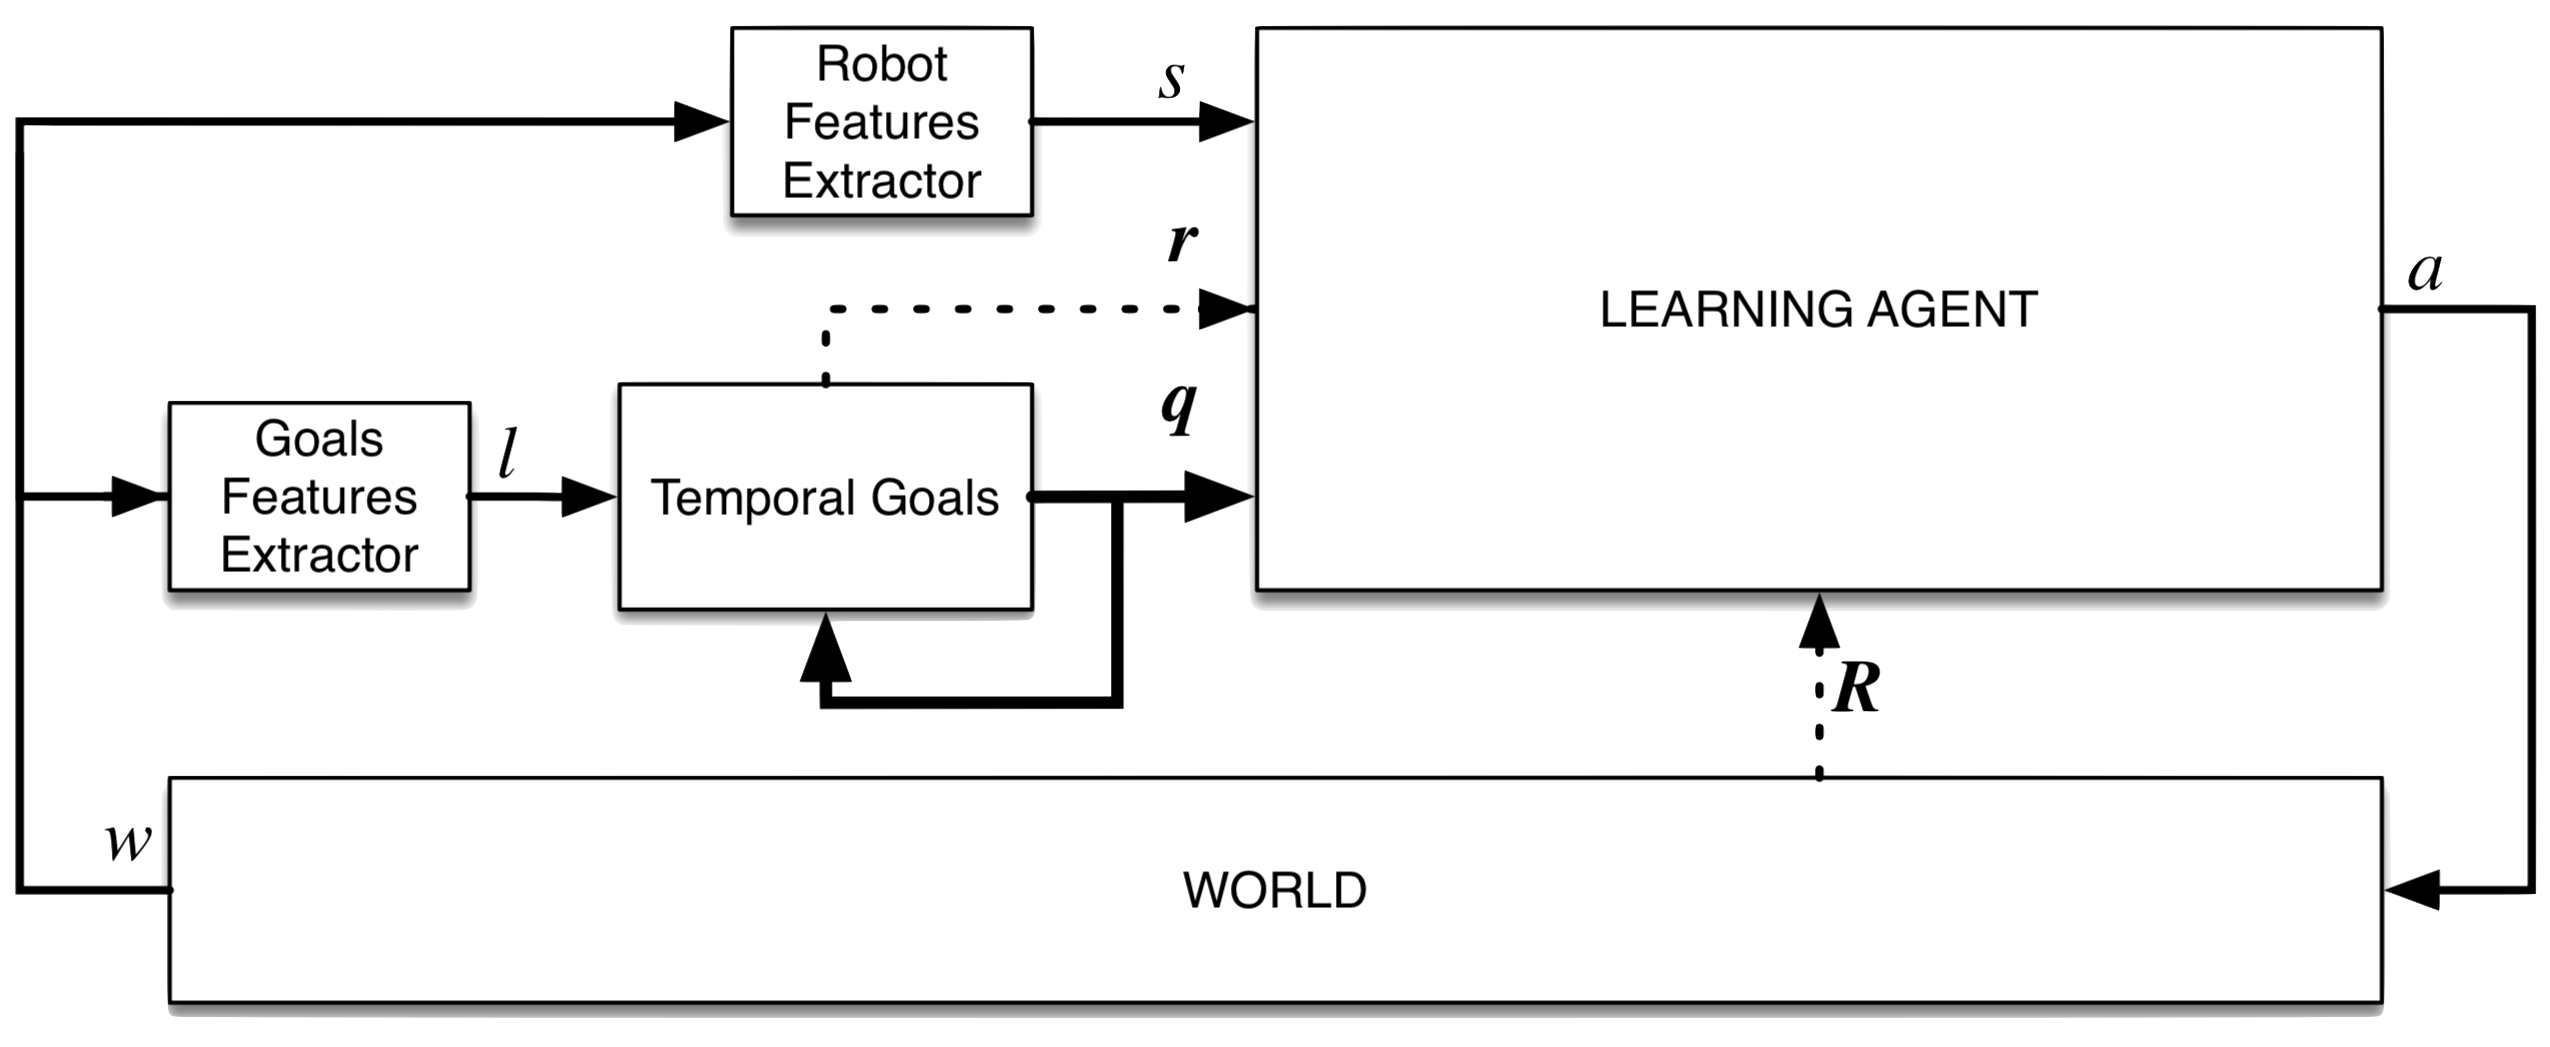
\includegraphics[width=0.95\textwidth]{images/rl-temporalgoals-pipeline.png}
        \caption{Pipeline describing how the agent is interacting with the
            world and how the robot features extractor and the goal features
            extractor are used in order to handle non-Markovian rewards.}
        \label{fig:rl-temporalgoals-pipeline}
    \end{figure}
\end{frame}

    \begin{frame}{PyGame Breakout}
	\begin{block}{}
	Starting from the work presented in \cite{DBLP:journals/corr/abs-1807-06333} the agents were trained on a modified PyGame Breakout with a $6\times18$ grid.
	\end{block}
	
	\begin{block}{}
	Game state already stored inside the class instance (ball position, paddle position, blocks status).
	\end{block}
	
\end{frame}

\begin{frame}{Atari Breakout}
    \begin{columns}[c,onlytextwidth]
        \column{0.65\textwidth}
	        \begin{block}{}
            Breakout from OpenAI Gym: toolkit for comparing learning algorithm. Provides easy access to state and reward. No assumption on the agent.
            \end{block}
        
	        \begin{block}{}
	        	Class stores pixels status. Need to extract information about the game state from it.
	        \end{block}

            \begin{block}{}
	            The environment is more stochastic.
			\end{block}
		
        \column{0.3\textwidth}
            \begin{figure}
                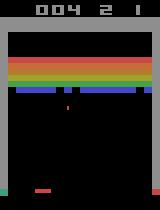
\includegraphics[width=\textwidth]{images/gym-breakout-image-example.jpg}
            \end{figure}
    \end{columns}
\end{frame}

    \section{Implementation}

\begin{frame}{Robot Features Extraction}
    Algorithms.
\end{frame}

\begin{frame}{Goal Features Extraction}
    Algorithms.
\end{frame}

\begin{frame}{Temporal Goals}
    Algorithms.
\end{frame}

    \section{Experiments}

\begin{frame}{Experiments}
    \begin{itemize}
        \item Example of gameplay in the Atari Environment
        \item This gameplay is the one that gave the best results, with a score of 63
        \item It's worth noting that the ball changes color when it's inside the brick area
    \end{itemize}
    \begin{columns}[c,onlytextwidth]
        \column{0.3\textwidth}
        \begin{figure}
            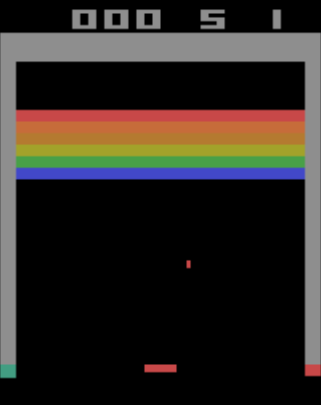
\includegraphics[width=\textwidth]{images/atari-sequence-0.png}
        \end{figure}
        %\hfill
        \column{0.3\textwidth}
        \begin{figure}
            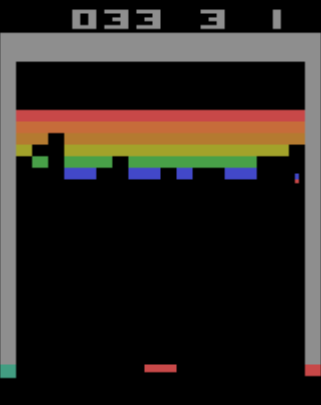
\includegraphics[width=\textwidth]{images/atari-sequence-1.png}
        \end{figure}
        %\hfill
        \column{0.3\textwidth}
        \begin{figure}
            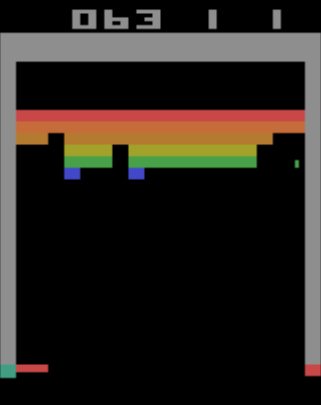
\includegraphics[width=\textwidth]{images/atari-sequence-2.png}
        \end{figure}
        %\caption{Sampled frames from the Atari Environment experiments}
    \end{columns}
\end{frame}

\begin{frame}{Experiments}
    \begin{columns}[c,onlytextwidth]
        \column{0.4\textwidth}
            \begin{figure}
                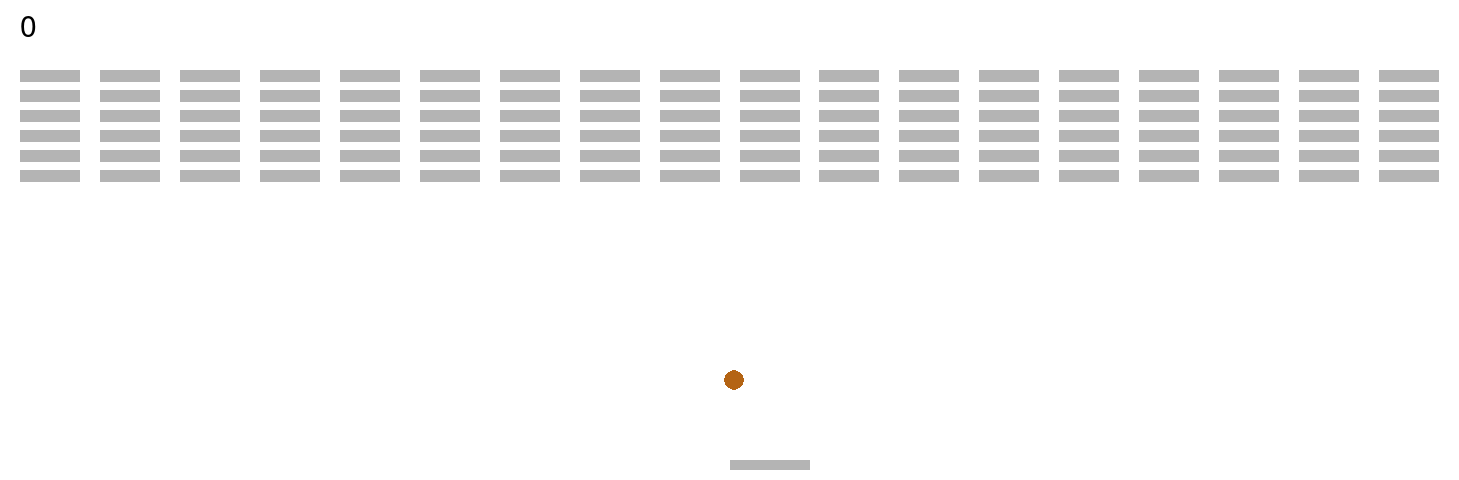
\includegraphics[width=\textwidth]{images/pygame-sequence-0.png}
            \end{figure}
            \begin{figure}
                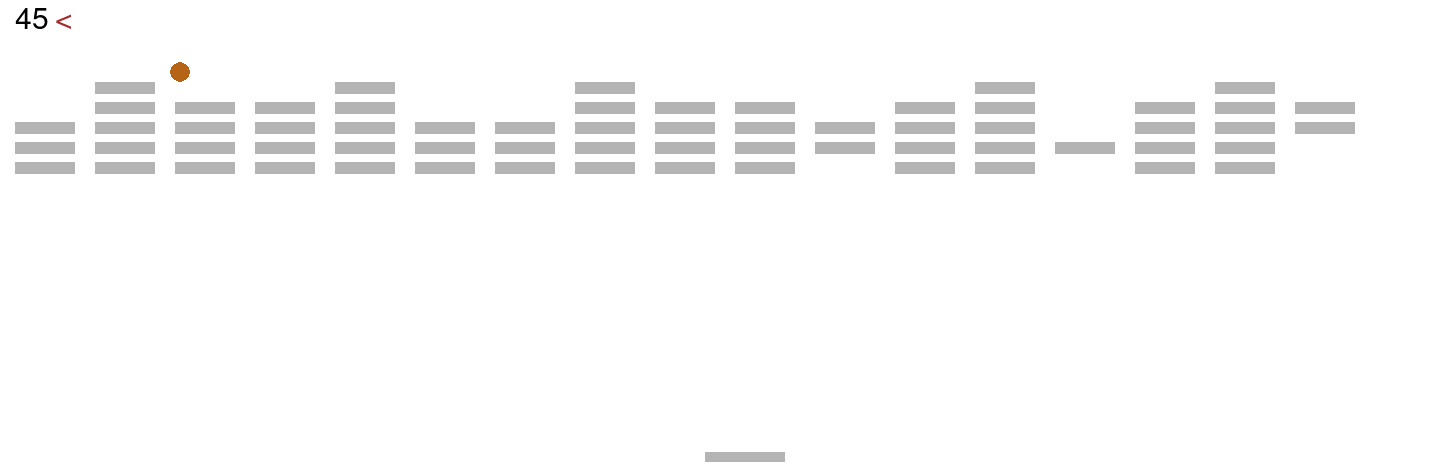
\includegraphics[width=\textwidth]{images/pygame-sequence-1.png}
            \end{figure}
            \begin{figure}
                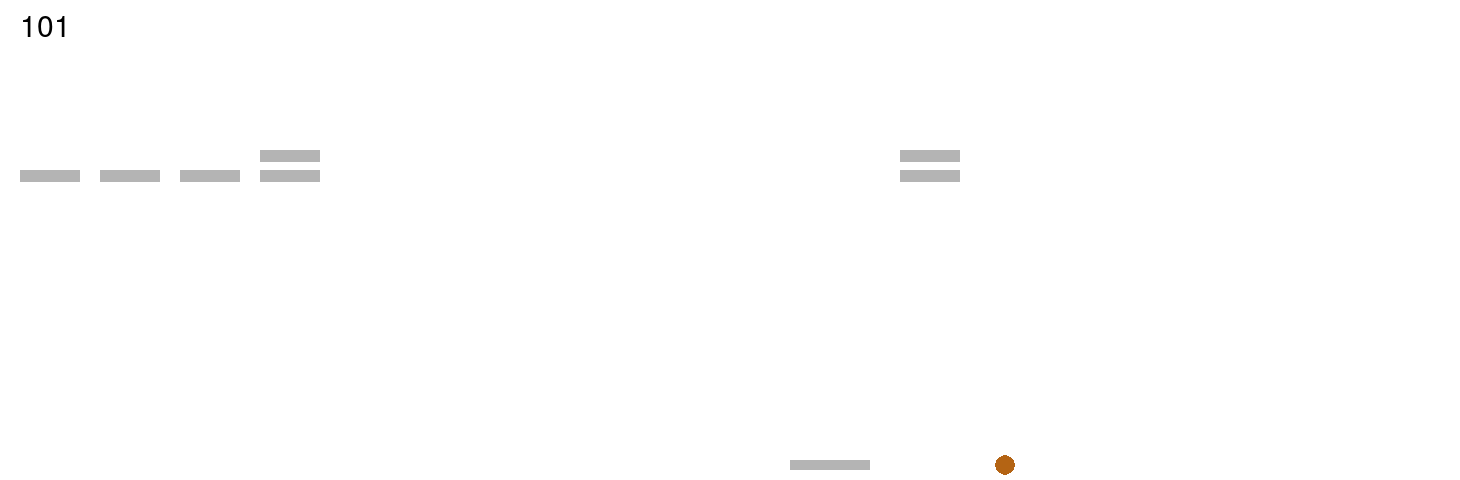
\includegraphics[width=\textwidth]{images/pygame-sequence-2.png}
            \end{figure}
        \column{0.6\textwidth}
	    \begin{itemize}
		\item Example of gameplay in the PyGame Environment
		\item This gameplay gave a score of 101
		\item In this case the ball does not change color, which is a further simplification compared to the Atari environment
		\item The window width/height ratio is much greater, but the ball is much slower
	    \end{itemize}
    \end{columns}
\end{frame}

\begin{frame}{Results}
	\begin{table}[h]
		\centering
		\begin{tabular}{*{8}{c}}
			Environment & Epochs & Explored States & Total Reward \\
			\hline
			Atari & 100,000 & 26,291 & 46 \\
			Atari & 200,000 & 26,271 & 63 \\
			\hline
			PyGame & 50,000 & 91,821 & 1010 \\
		\end{tabular}
	\end{table}
	    \begin{itemize}
		\item Comparison of the results obtained
		\item All the tests shown above were performed with the SARSA algorithm
		\item It is important to note that the reward is assigned differently in the two environments
		\item PyGame returns a reward of 10 for the destruction of any brick
		\item Atari returns a reward equal to 1, 4 or 7 for the destruction of a brick
	    \end{itemize}
\end{frame}

\begin{frame}{Atari Environment results}
    \begin{columns}[c,onlytextwidth]
        \column{0.5\textwidth}
            \begin{figure}
                \centering
                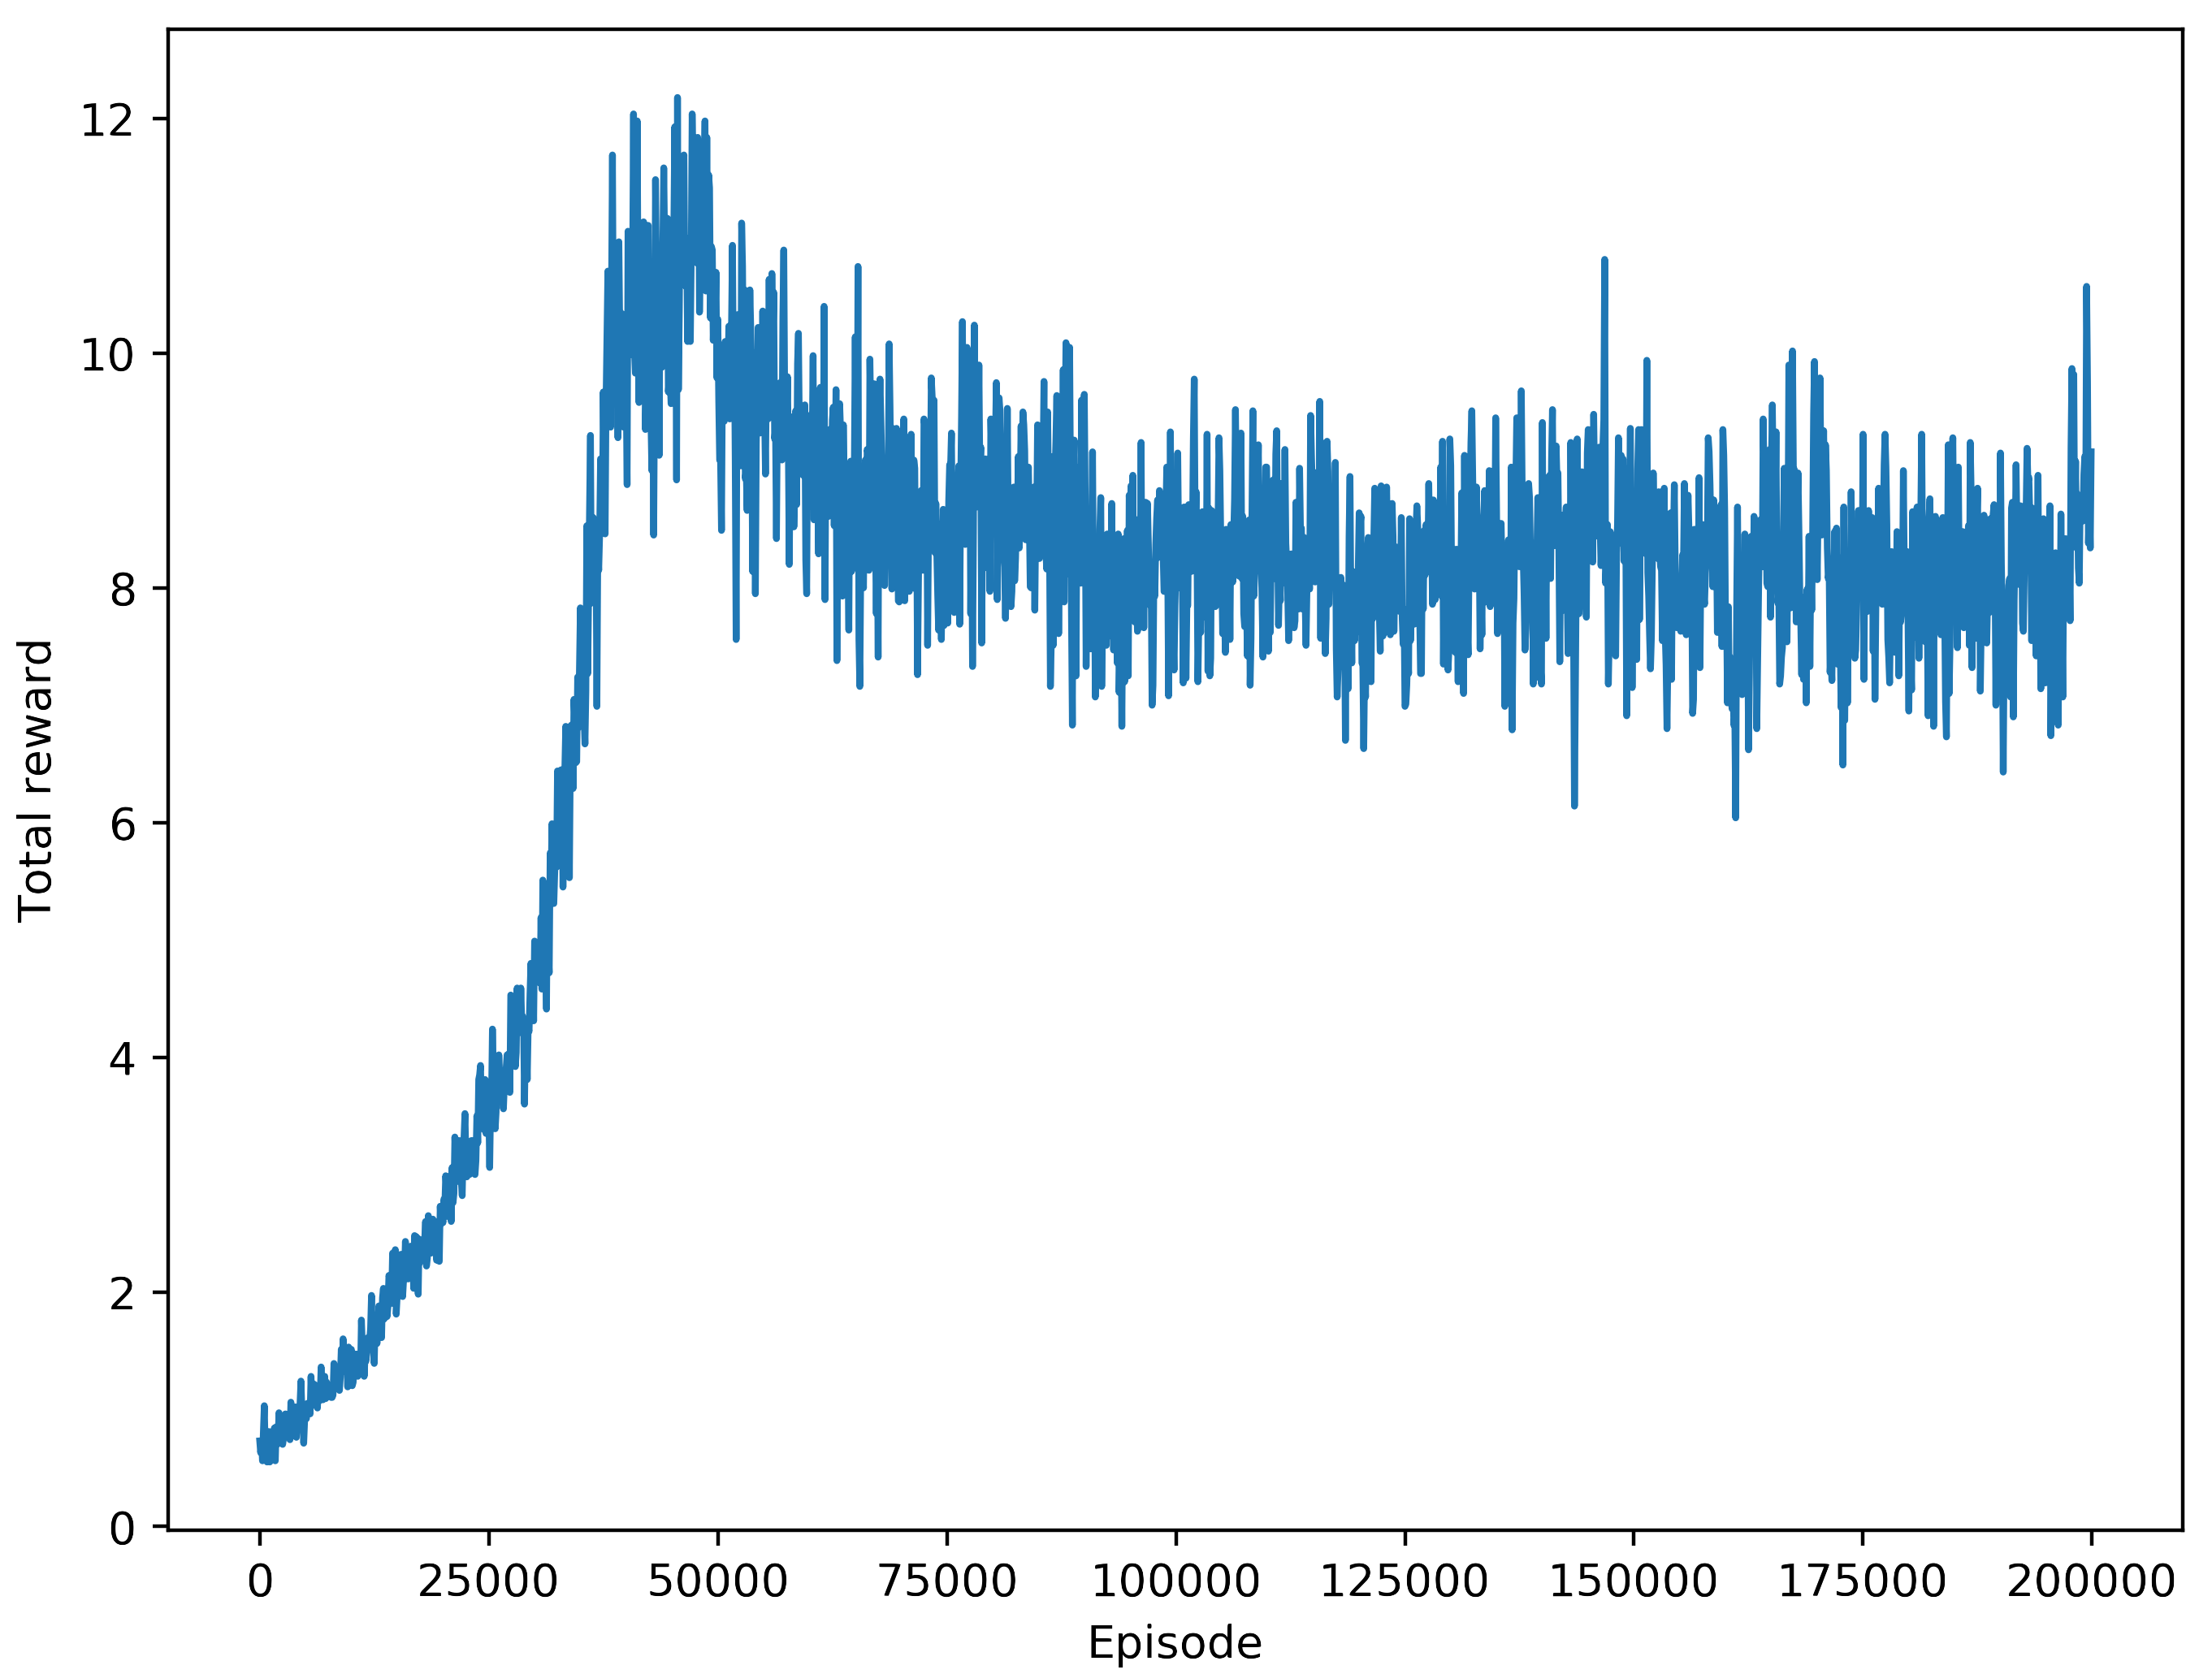
\includegraphics[width=0.8\textwidth]{images/atari-ql-total-reward.png}
            \end{figure}
            \begin{figure}
                \centering
                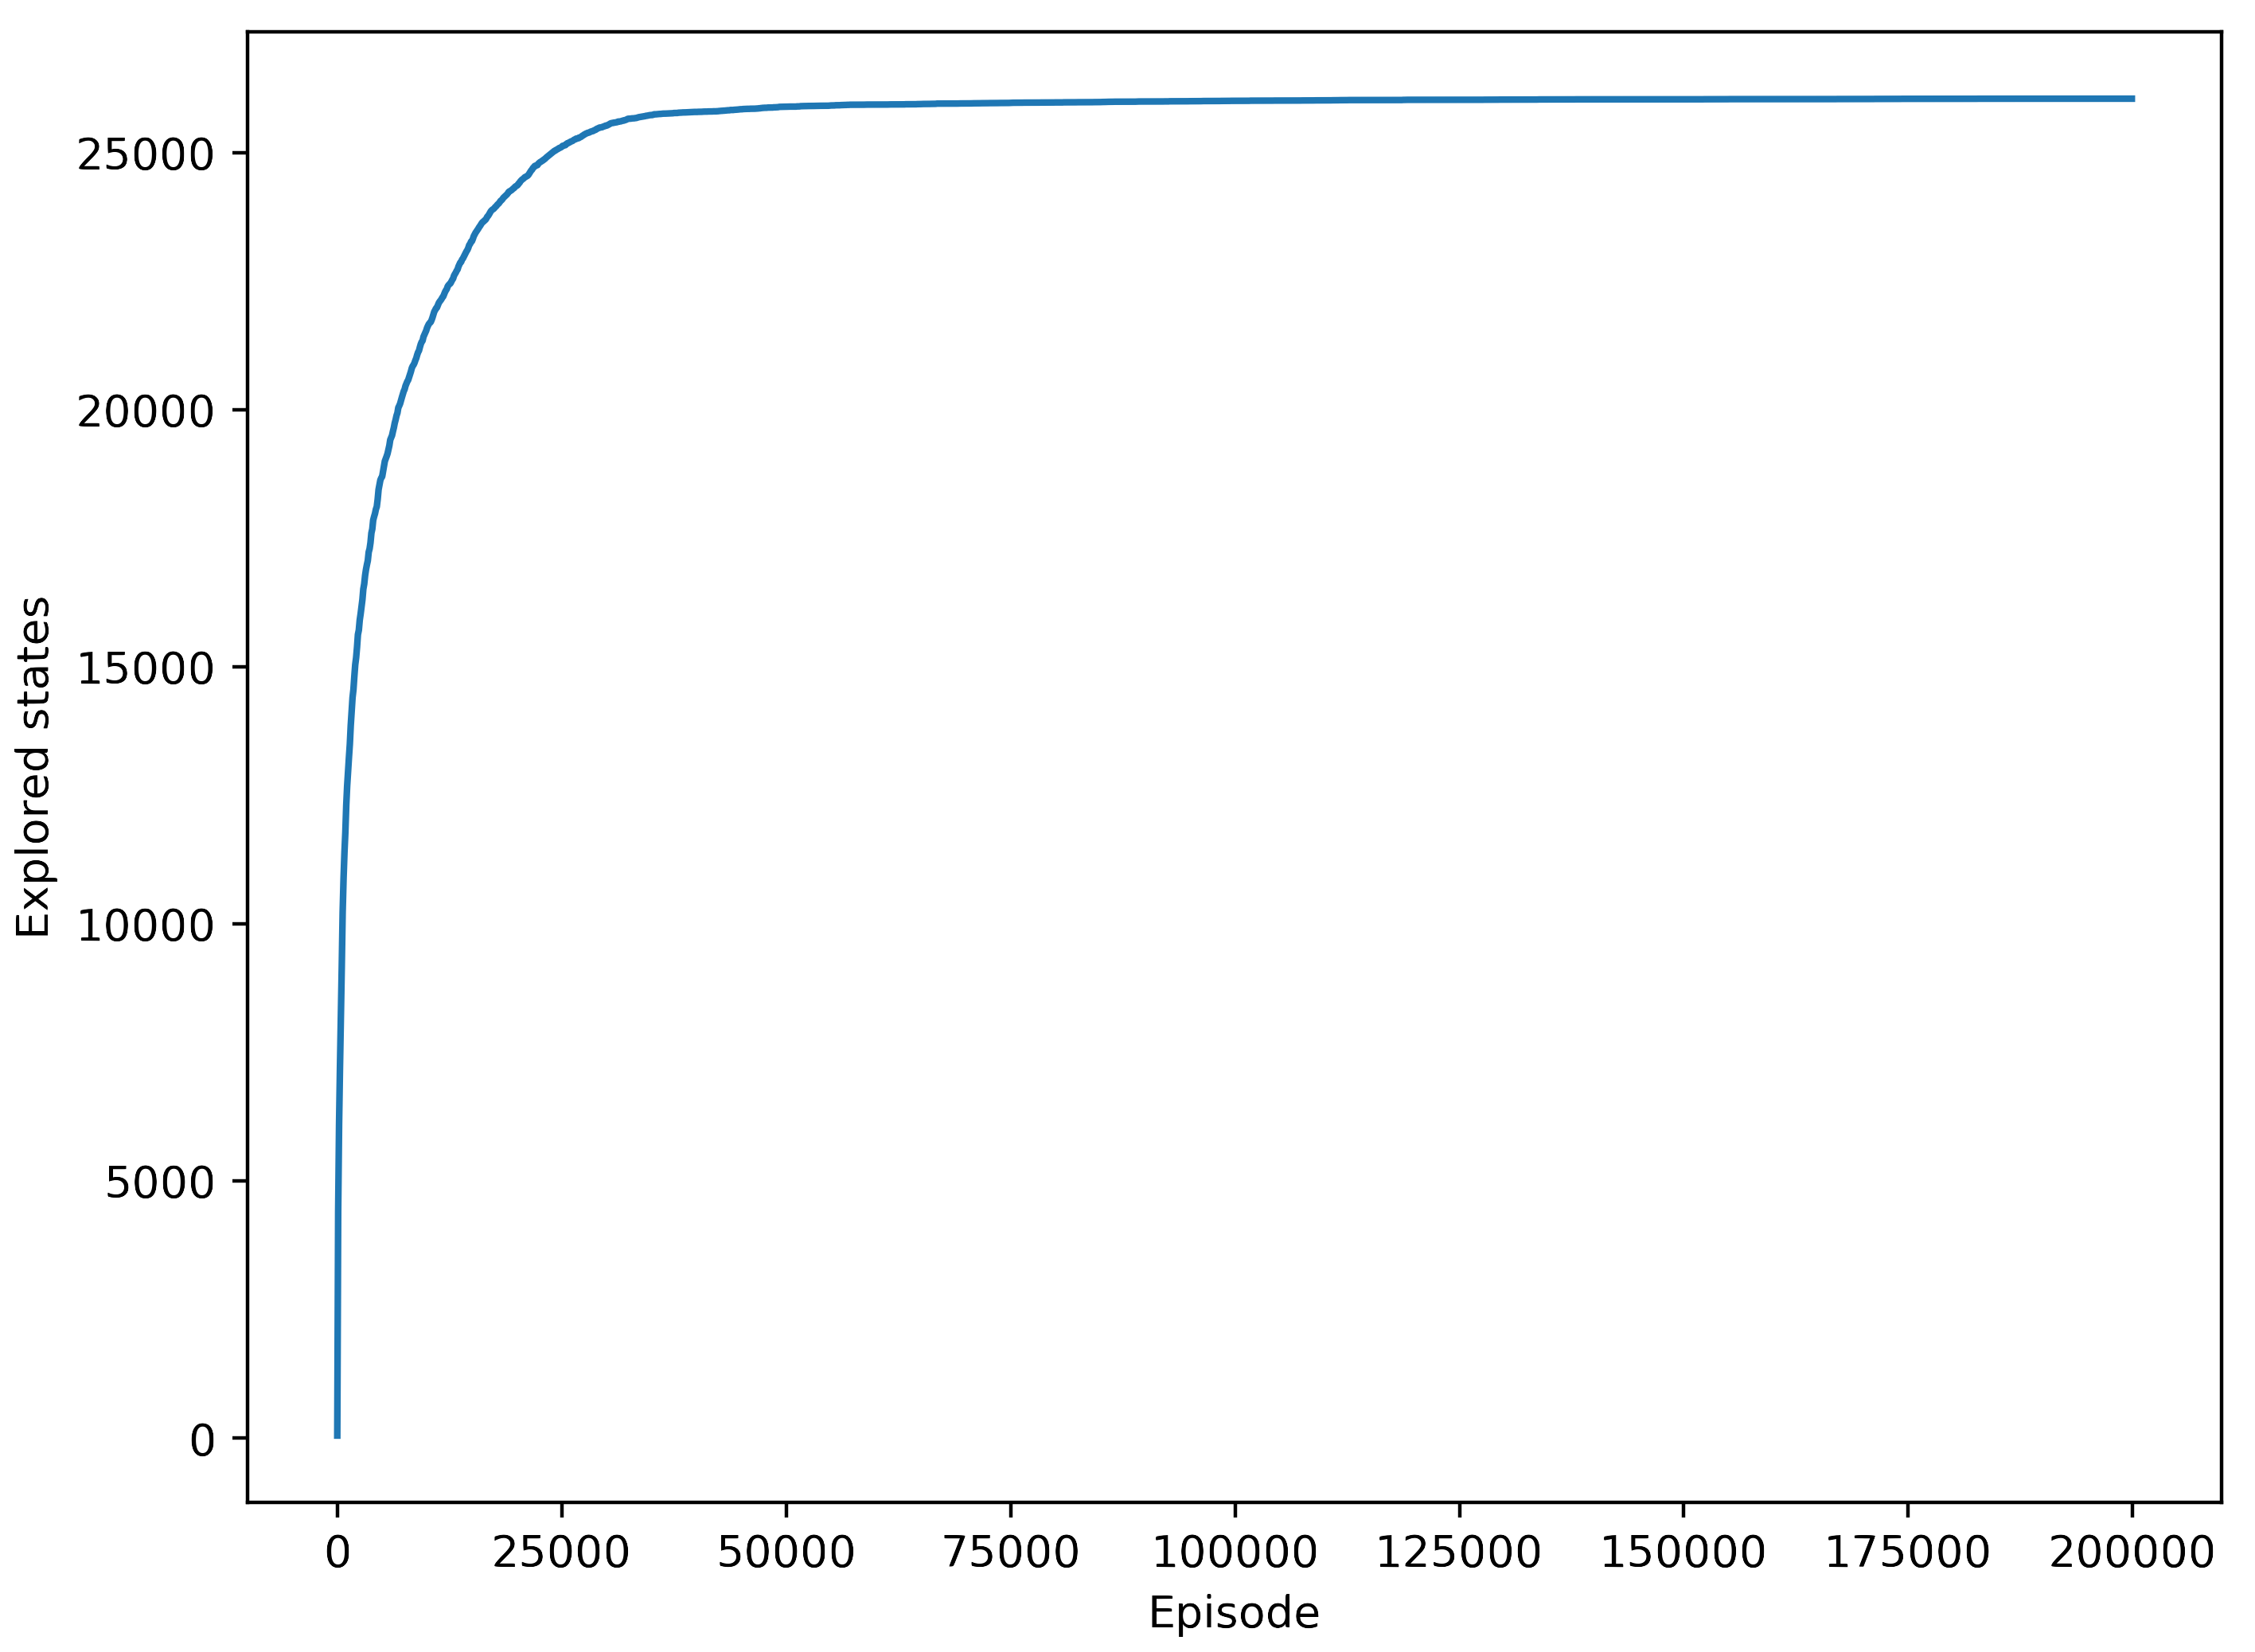
\includegraphics[width=0.8\textwidth]{images/atari-ql-explored-states.png}
		\caption{Q-Learning algorithm}
            \end{figure}
        \column{0.5\textwidth}
            \begin{figure}
                \centering
                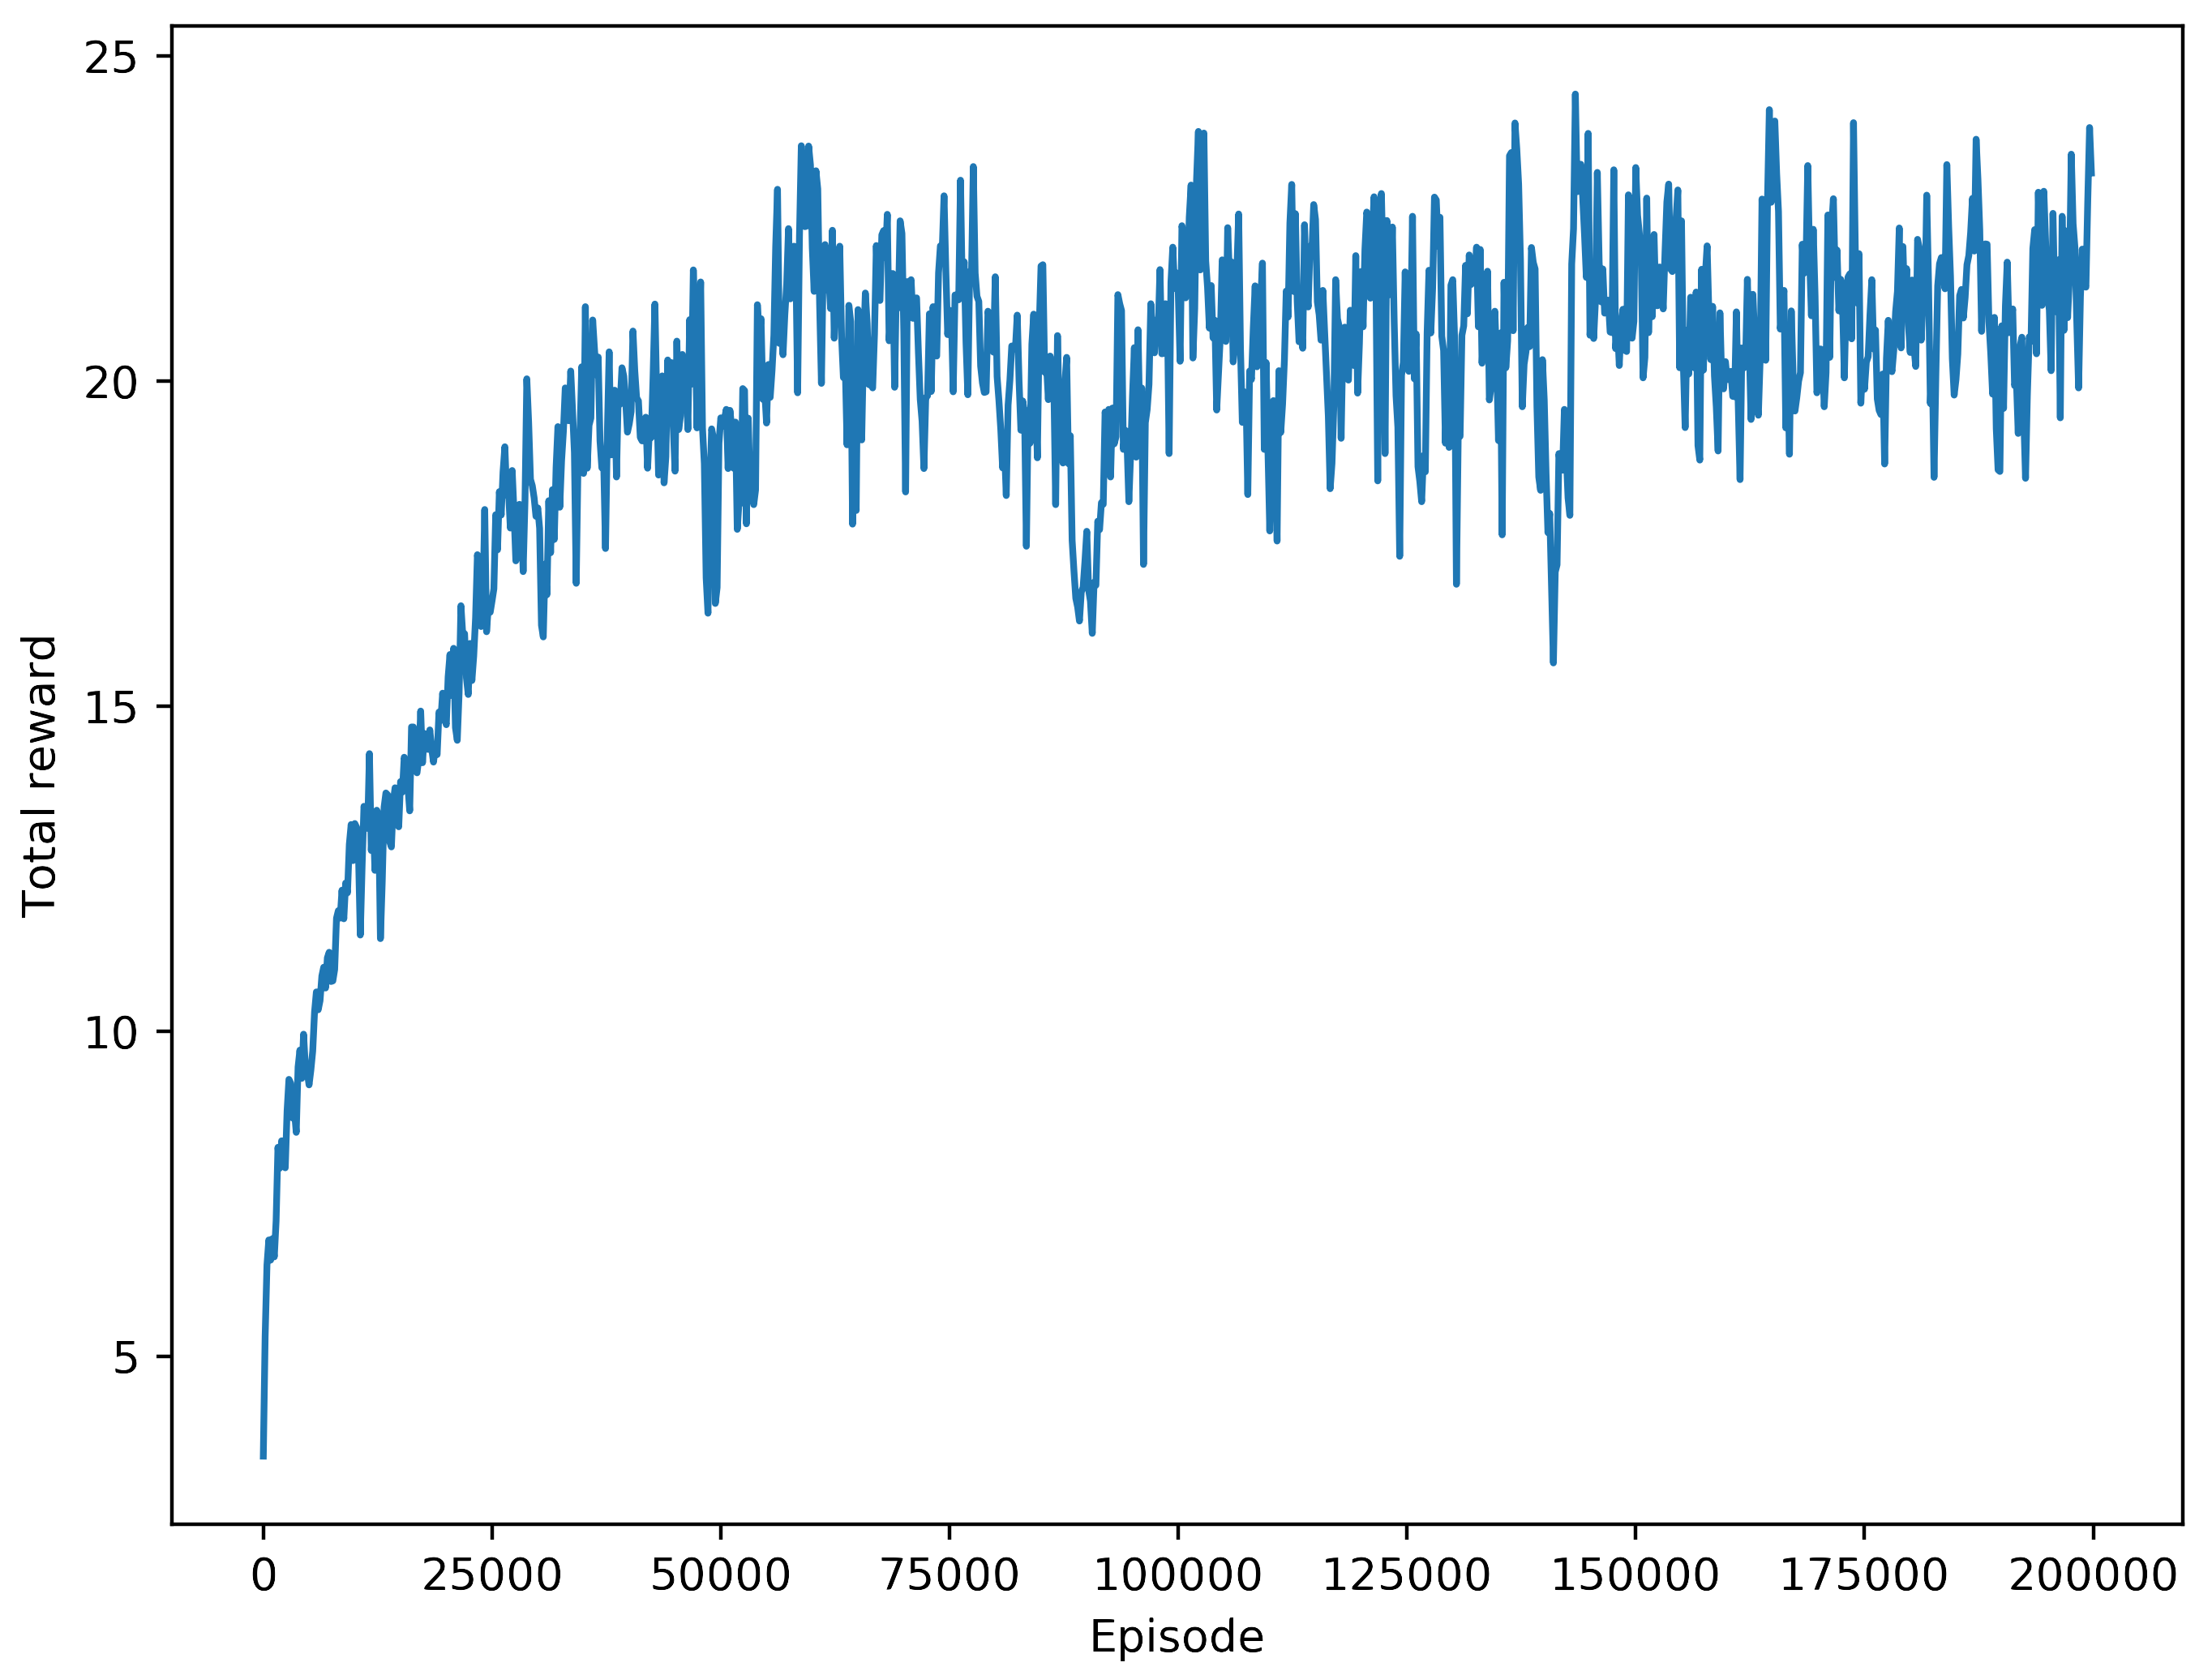
\includegraphics[width=0.8\textwidth]{images/atari-sarsa-total-reward.png}
            \end{figure}
            \begin{figure}
                \centering
                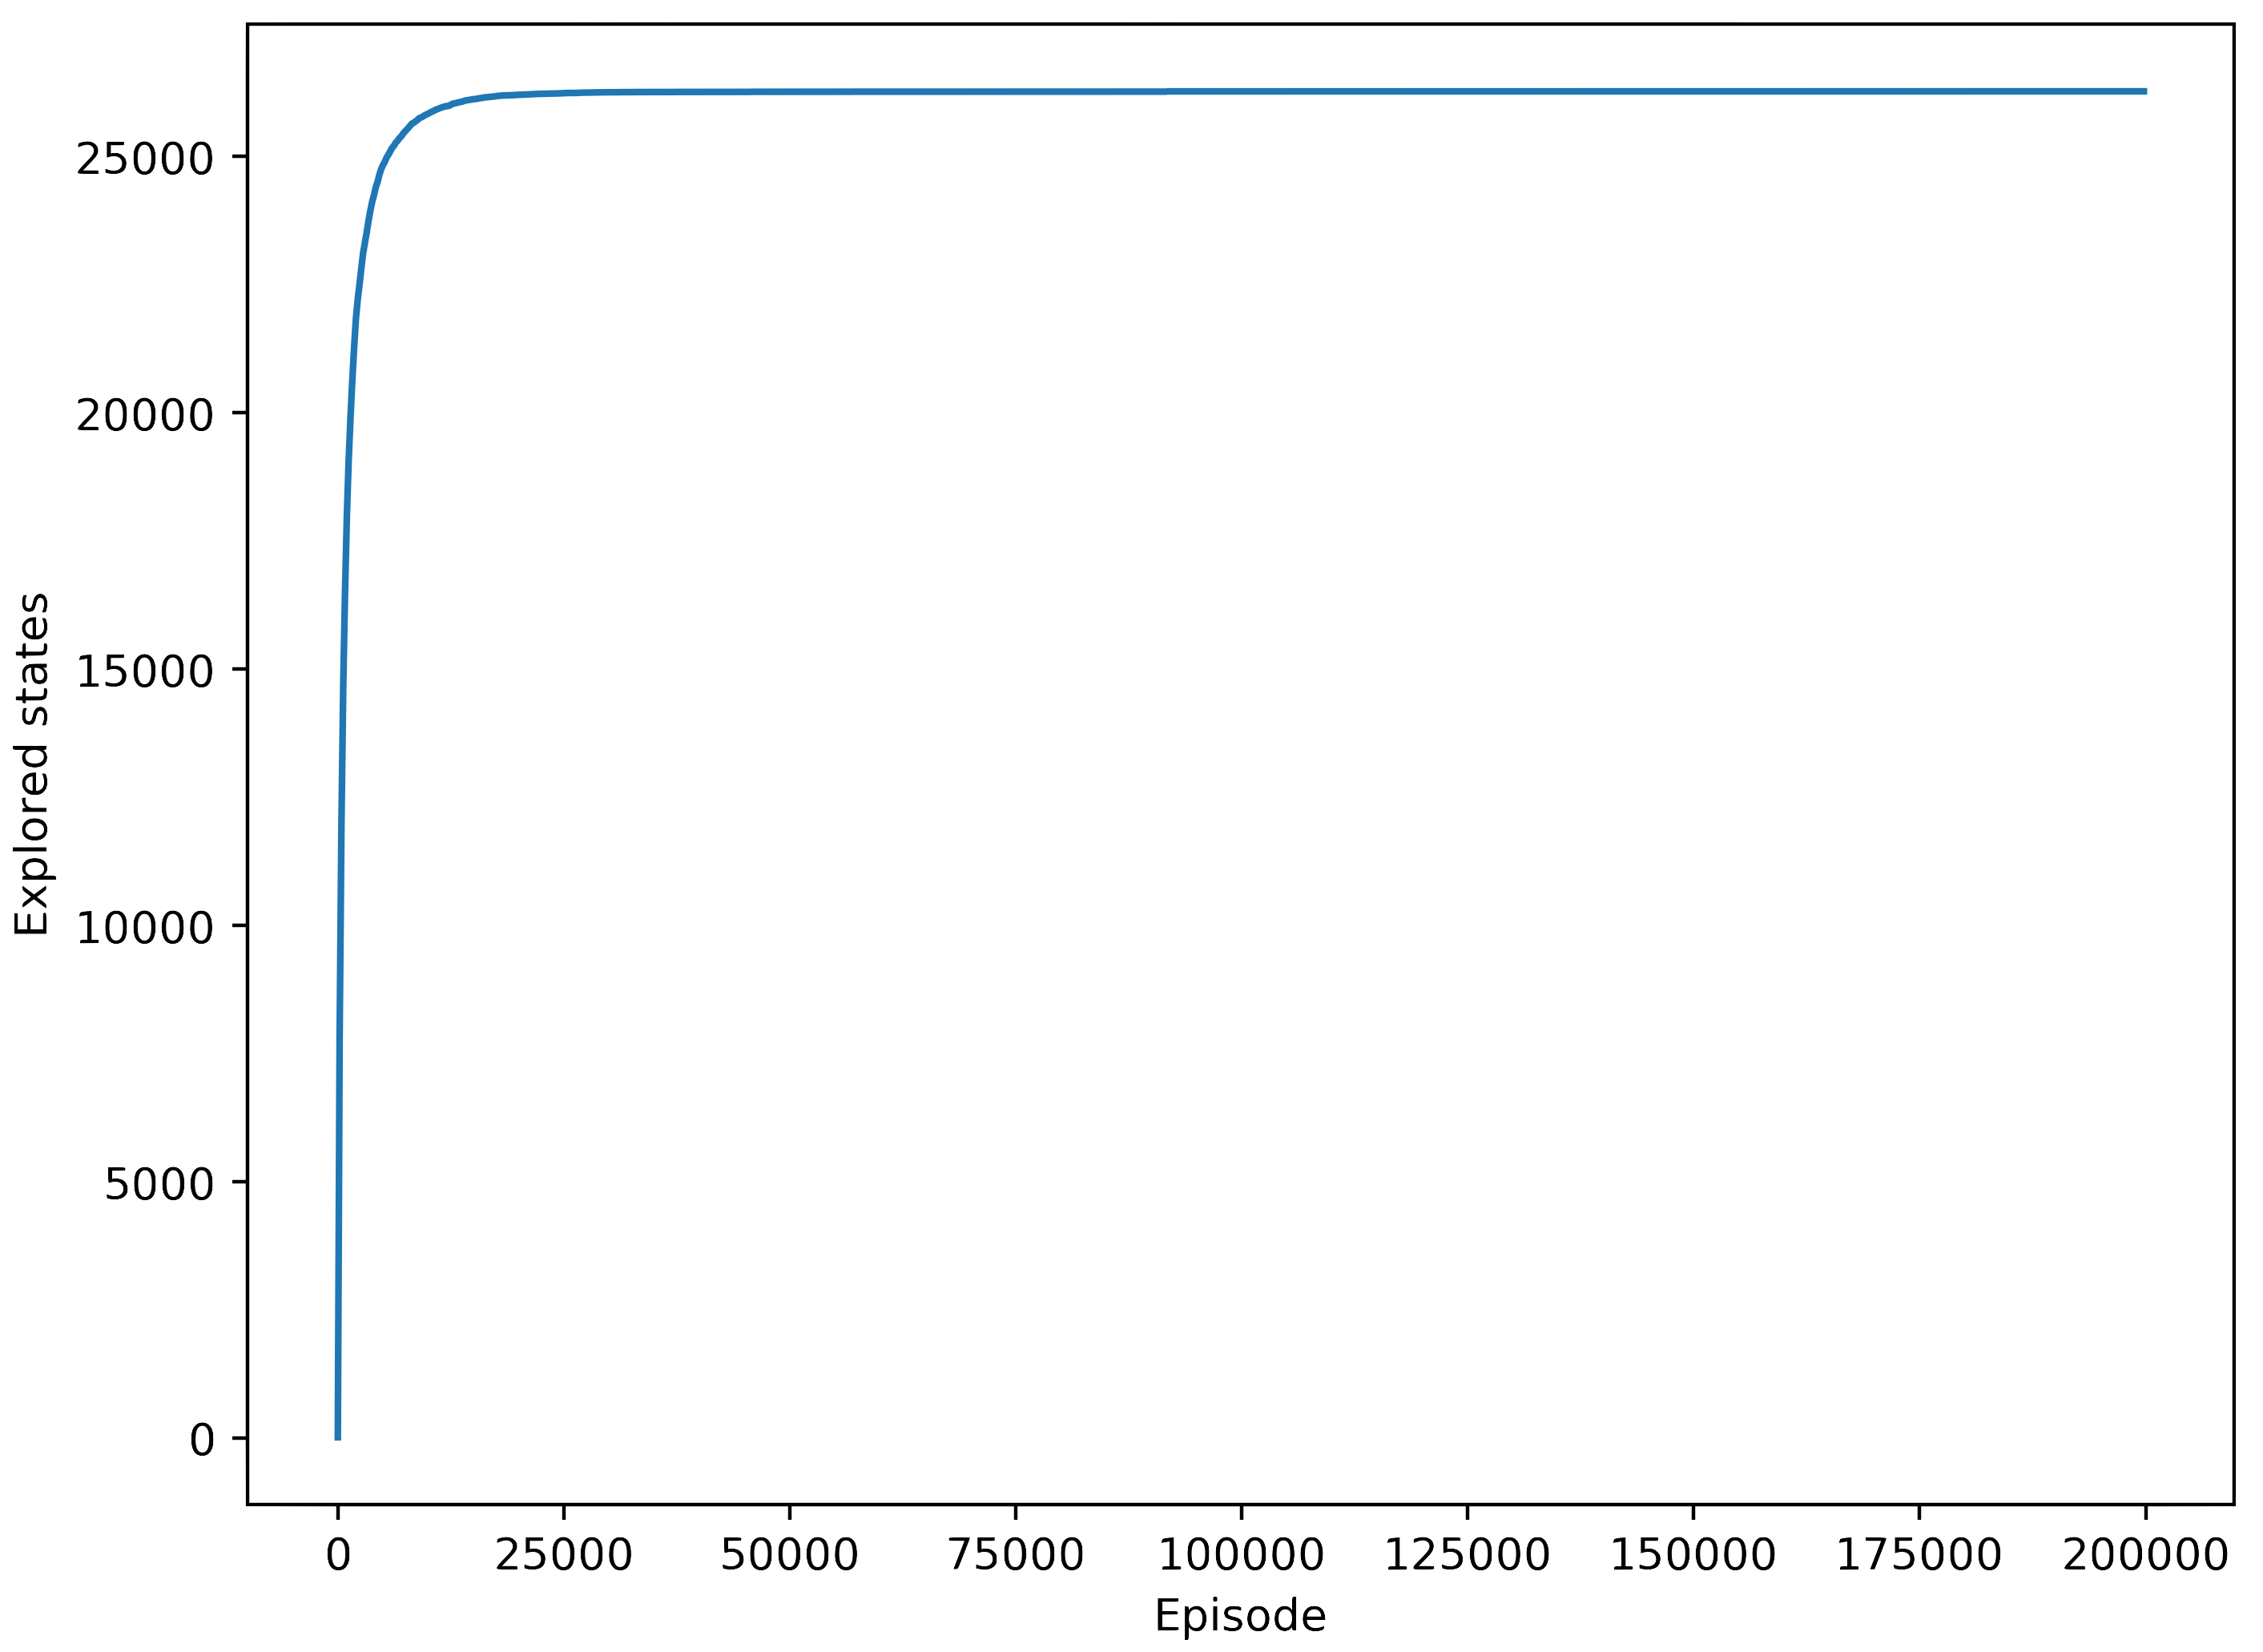
\includegraphics[width=0.8\textwidth]{images/atari-sarsa-explored-states.png}
		\caption{SARSA algorithm}
            \end{figure}
    \end{columns}
\end{frame}

\begin{frame}{PyGame Environment results}
    \begin{columns}[c,onlytextwidth]
        \column{0.4\textwidth}
            \begin{figure}
                \centering
                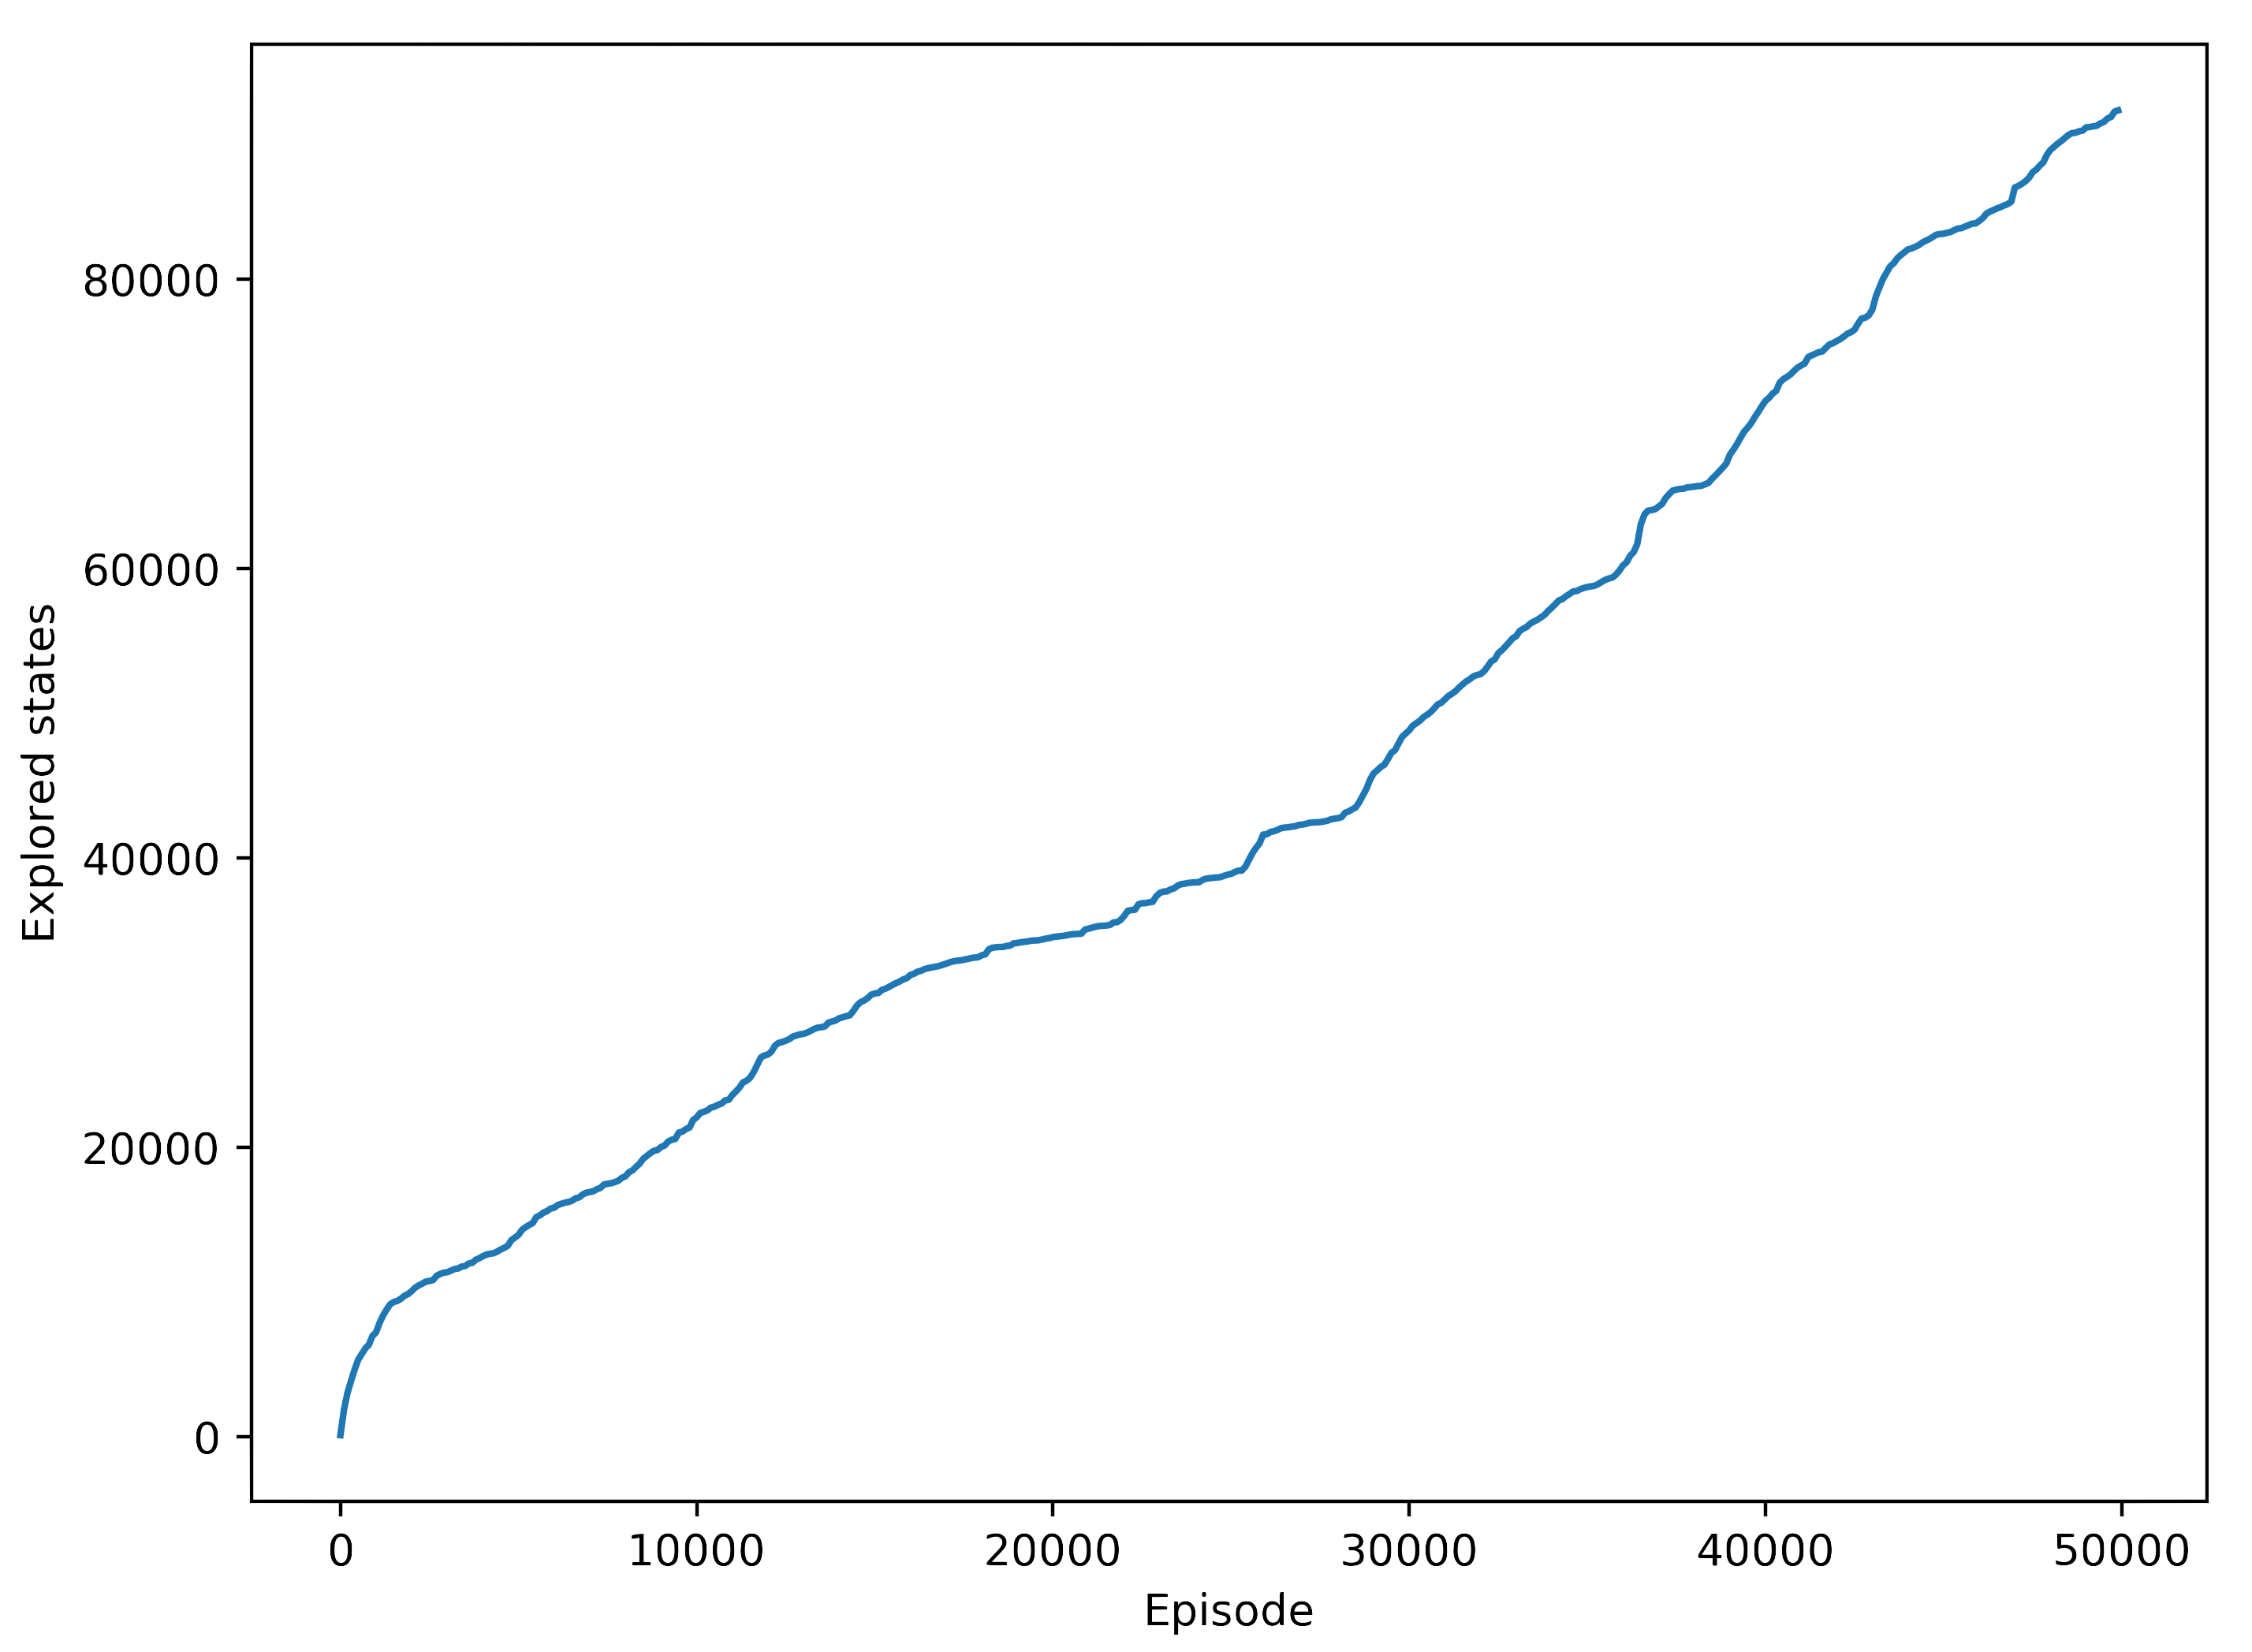
\includegraphics[width=\textwidth]{images/pygame-explored-states.png}
            \end{figure}
            \begin{figure}
                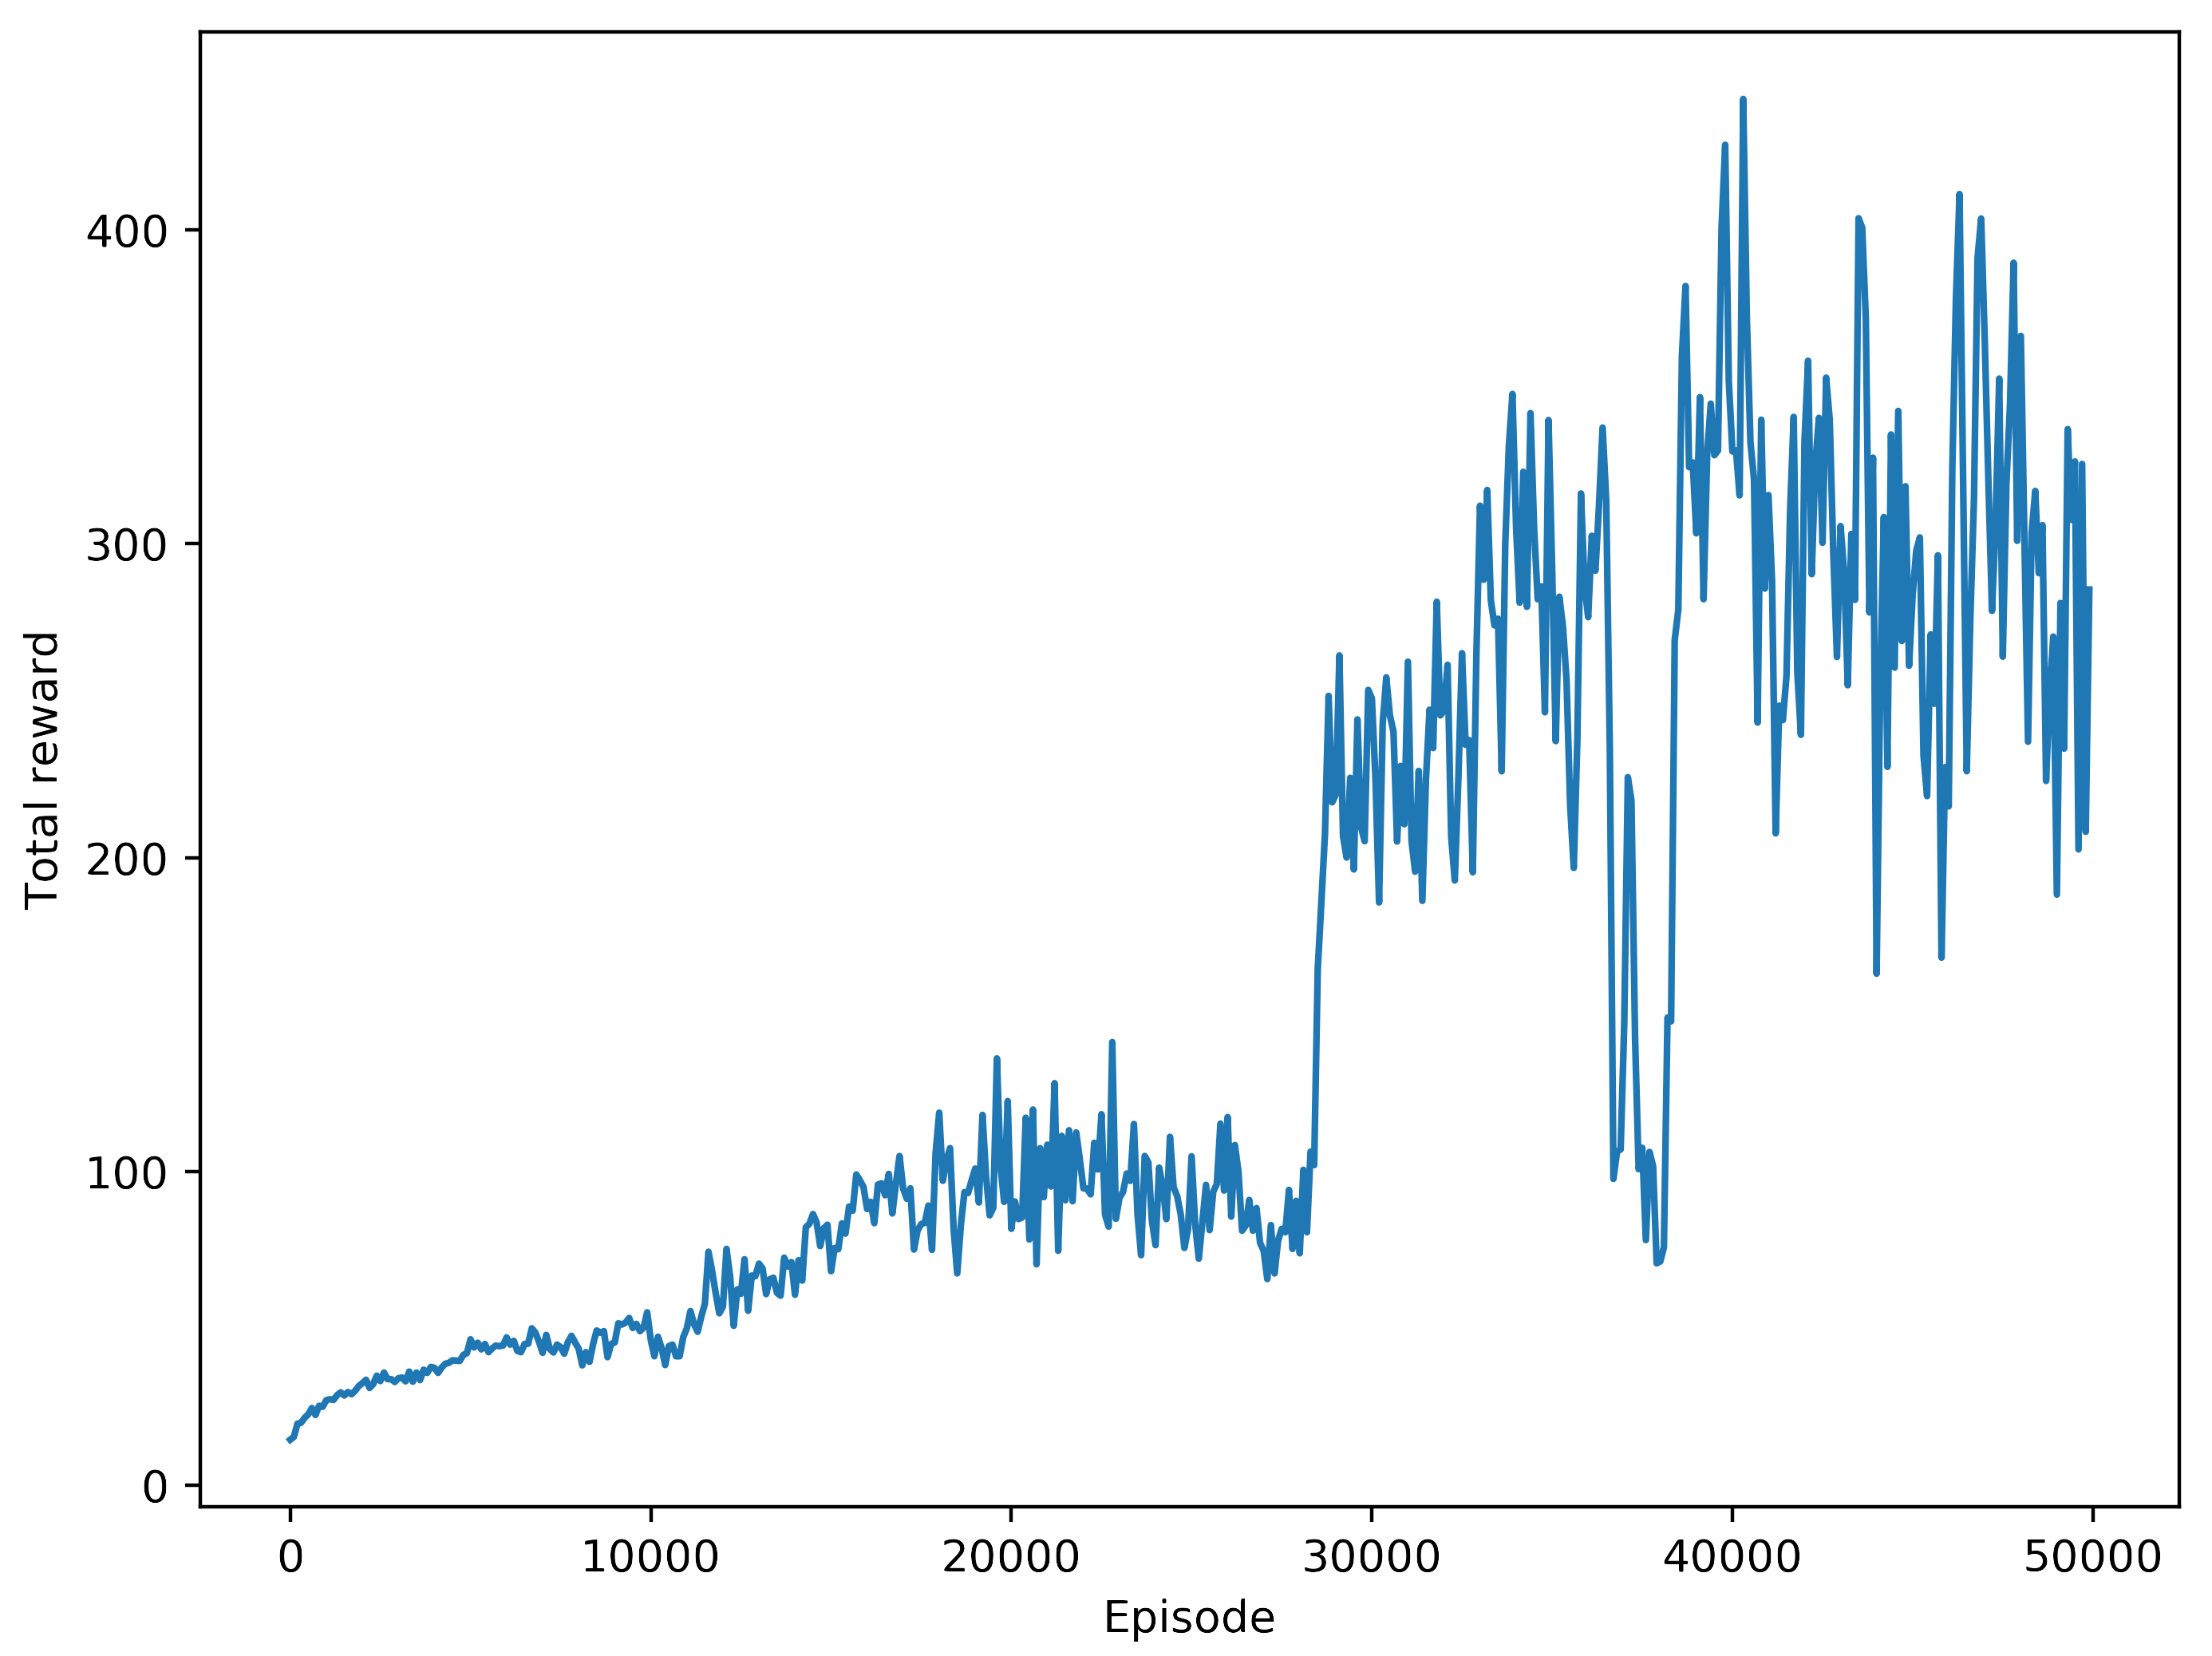
\includegraphics[width=\textwidth]{images/pygame-total-reward.png}
            \end{figure}
        \column{0.6\textwidth}
	    \begin{itemize}
		\item The Total Reward in the PyGame Environment is much higher
		\item In the Atari Environment, the number of states explored has stabilized after 25,000 epochs
		\item In the Pygame Environment, the number of states explored shows an increasing linear trend along the entire sample of 50,000 epochs
		\item The number of states explored in PyGame exceeds 90,000, a sign that the game continues to move forward, exploring more and more states
	    \end{itemize}
    \end{columns}
\end{frame}

\begin{frame}{The Modified PyGame}
    \begin{itemize}
	\item We tried to investigate what was going on
	\item The paddle-bricks distance is covered in 35 frames in PyGame, only 15 in Atari
	\item In 1500 frames, the agent manages to destroy 10 bricks in PyGame, 29 in Atari
	\item In the Atari Environment there are 5 lives, but only 1 in PyGame
	\item Given alle the differences, we changed the two environments to make them as similar as possible, to compare them better
    \end{itemize}
    \begin{figure}
        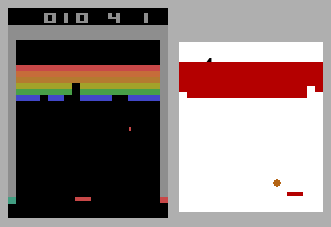
\includegraphics[width=0.5\textwidth]{images/modified-pygame-comparison.png}
    \end{figure}
\end{frame}

\begin{frame}{A Better Comparison}
The pygame environment thus modified was able to learn the destruction of an entire line already from 5,000 epochs.

\bigskip
The Atari environment, on the other hand, could not achieve this goal even after 200,000 eras.

\bigskip
But these tests produced interesting results
\end{frame}

\begin{frame}{Tests}
\begin{small}
	\begin{table}[h]
		\centering
		\begin{tabular}{*{8}{c}}
			Ball X & Ball Y & Angle & Paddle & Move & Lives Count & Frame Skip & Score \\
			\hline
			144 & 157 & 10 & 144 & 49 & 1 & 4 & 6 \\
			144 & 157 & 10 & 144 & 49 & 5 & 4 & 4-20 \\
			8 & 18 & 10 & 8 & 49 & 1 & 4 & 5 \\
			144 & 157 & 10 & 144 & 10 & 1 & 4 & 7 \\
			144 & 157 & 10 & 144 & 0 & 1 & 4 & 7 \\
			144 & 157 & 10 & 144 & 0 & 5 & 4 & 2-16 \\
			8 & 18 & 10 & 8 & 10 & 1 & 4 & 6 \\
			8 & 18 & 10 & 8 & 0 & 1 & 4 & 2 \\
			8 & 18 & 10 & 8 & 0 & 5 & 4 & 5-15 \\
			\hline
			144 & 157 & 10 & 144 & 13 & 5 & 14 & 19 \\
			144 & 157 & 10 & 144 & 13 & 5 & 10 & 24 \\
			144 & 157 & 10 & 144 & 13$^1$ & 5 & 10 & 16 \\
			144 & 157 & 10 & 144 & 121 & 5 & 10 & 24 \\
		\end{tabular}
		\caption{$^1$ This test was performed with the same hyperparameters as the previous test, but with a different calculation of the move variable: instead of distributing the 13 states of the move variable from -60 to +60 motion pixels, they were distributed over the range [-40 , +40], cropping excess values.}
	\end{table}
\end{small}
\end{frame}

\begin{frame}{The Atari Breakout Difficulties I}
\textbf{The Dimension Space Problem}
    \begin{itemize}
	\item Many tests have been carried out to reduce the space of states in Atari
	\item Many tests have been carried out to reduce the space of states in Atari
	\item Some even showed a worsening effect
	\item The algorithm fails to learn from the states it has visited
	\item There is therefore a deep problem in the Atari Environment
    \end{itemize}
\end{frame}

\begin{frame}{The Atari Breakout Difficulties II}
\textbf{The Local Maximum Problem}
    \begin{itemize}
	\item There are many states from which it is difficult to escape
	\item If the paddle is in the corner it will be very difficult to get out of it
	\item Increasing the number of frameskip alleviates this problem, but increases the problem of non-determinism
    \end{itemize}
	\begin{figure}
		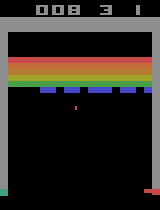
\includegraphics[width=0.19\textwidth]{images/frame-sequence-0.png}
		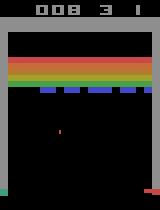
\includegraphics[width=0.19\textwidth]{images/frame-sequence-1.png}
		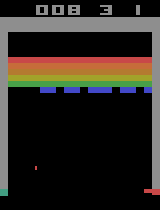
\includegraphics[width=0.19\textwidth]{images/frame-sequence-2.png}
		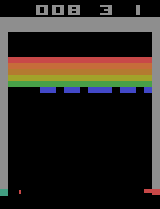
\includegraphics[width=0.19\textwidth]{images/frame-sequence-3.png}
		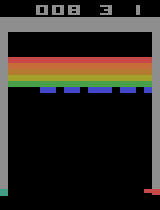
\includegraphics[width=0.19\textwidth]{images/frame-sequence-4.png}
		\caption{Sequence of sampled frames}
	\end{figure}
\end{frame}

\begin{frame}{The Atari Breakout Difficulties III}
\textbf{The Non-Determinism Problem}
    \begin{itemize}
	\item The real problem that has constituted the main obstacle is the non-determinism of the paddle
	\item The paddle movement consists of two parts: a random part and an inertial part
	\item A variable called \text{move} in the statespace was added to alleviate the inertial part 
	\item The random part can not be resolved, and is the cause of the last problem:
    \end{itemize}
\end{frame}

\begin{frame}{The Atari Breakout Difficulties IV}
\textbf{The State Collision Problem}
    \begin{itemize}
	\item Because of non-determinism, some different situations share the same states
	\item This means that when two similar situations happen in the same game, conflicts can occur
	\item The best action in the first of two states may not be the best action in the second state
	\item When the agent learns the best action of the second state, he overwrites the first state, losing all the progress made up to that point
	\item This makes training for reinforcement learning on the Atari Environment extremely difficult
    \end{itemize}
\end{frame}

    \begin{frame}{Conclusion}
    \begin{itemize}
	\item The presented project is an extension of the previous project on the Atari Environment
	\item The best performance did not manage to correctly solve the Atari Breakout game
	\item Fundamental problems have been identified, in particular non-determinism, in the environment
	\item Those problems prevent algorithms such as Q-Learning or SARSA from achiving satisfactory results
	\item Future work must be done to solve such problems, especially the introduction of a neural network
    \end{itemize}
\end{frame}


    \begin{frame}[standout]
        Q\&A
    \end{frame}

    \appendix

    \begin{frame}[allowframebreaks]{References}
        \bibliography{bibliography}
        \bibliographystyle{ieeetr}
    \end{frame}

\end{document}
